\chapter{Experiment and Evaluation - System Performance}
\section{Goals}
This experiment is like a proof of concept to show that Graphy's data models for tags and relationships can be exchanged and synchronized between mobile clients like other Contacts application with similar performance. The goals of the experiment are as follows:

\begin{itemize}
    \item Clients can push contact data to backend server.
    \item Clients can pull contact data from backend server.
    \item Clients can synchronize their contact data with each other (through the help of the backend server).
    \item Clients can resolve contact data conflicts between each other (through the help of the backend server).
\end{itemize}

\section{Experimental Setups}
\subsection{Overview}
The experimental system basically contains three parts: the clients, the backend server, and the communication between them. Everything runs on a Macbook Pro 2012 with the specifications listed in \autoref{tb:specs}. The Macbook provides a Unix-like environment where we can run everything we need easily. However, compared with a real-world production system, our setup is slower by a huge margin. To be more specific, we use multi-threading programming in order to simulate multiple devices. For communication, we just run the clients and the backed server on the same local host. This method eliminates the delay of the actual Internet connection so we can focus on examining the synchronization process. Even though we can find better equipments, we decide to run our tests on this slow system, if the experiment yields good results, it means it will work even better on a more powerful environment.

\begin{table}[!ht]
\centering
\caption{System's Specifications}\label{tb:specs}
\begin{tabular}{ | c | l | }
\hline
	Processor & \specialcell{2.5GHz dual-core Intel Core i5\\(Turbo Boost up to 3.1GHz)\\with 3MB L3 cache} \\ \hline
	Memory & 8GB of 1600MHz DDR3 memory \\ \hline
	Storage & 500GB 5400-rpm hard drive \\ \hline
	Operating System & OSX Yosemite v.10.10\\ \hline
\end{tabular}
\end{table}

\subsection{Clients}
The actual fully-featured mobile clients are written in C\# on the Xamarin platform. However, in this experiment to reduce the manual tasks to a minimum we re-write the clients using multiple threads, each thread represents one client. We also discard all the unnecessary code like the user interface and other unrelated functions. The experiment code of clients can be accessed at: \url{https://github.com/NamXH/GraphyClient}, and the fully-functional mobile clients' code can be accessed at: \url{https://github.com/NamXH/GraphyPCL}. As a result, we take full controls of the client threads and we can trigger the synchronization process at any specific moment precisely. Moreover, using the asynchronous programming model with Async and Await in C\# we can run many client threads in parallel to simulate multiple devices being used at the same time. Besides, since we only test the performance of the data synchronization which operates on each user separatedly so for fast prototyping we do not implement authentication in the experiment.

On the other hand, the databases of the clients are carefully implemented for every thread. We also use SQLite which is the same technology as the mobile devices. The details of the database schema can be found in Appendix B. Regarding the Sync Queue, each modification on the database (creating/updating/deleting a business record) is mapped to a row in the Sync Queue table. For instance, a creation is mapped to a POST request, an update is mapped to a PUT request, and a deletion is mapped to a DELETE request. \autoref{fg:sync_queue} shows some examples of the Sync Queue table.

\begin{figure}[!h]
\begin{centering}
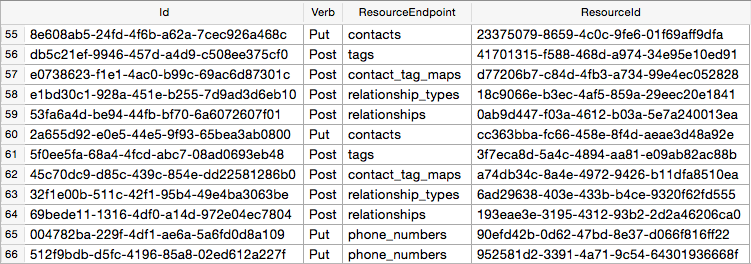
\includegraphics[scale=0.63]{pics/sync_queue.png}
\caption{Sync Queue Table}\label{fg:sync_queue}
\end{centering}
\end{figure}

\subsection{Server}
The backend server is written in Python using the Django framework. Its code can be accessed at: \url{https://github.com/NamXH/GraphyBackend}. \autoref{fg:server_implementation} presents some examples of the database models written for the server. We run the Python code on the Gunicorn web server with 5 workers because our processor has 4 cores. It is also worth mentioning that the server's database is implemented by using PostgreSQL - a high performance, open source, relational database. Python and Django have incredible support for PostgreSQL so the setup is very simple. Moreover, we can use the Python object-relational mapper to access PostgreSQL instead of writing raw SQL queries.

\begin{figure}[!h]
\begin{centering}
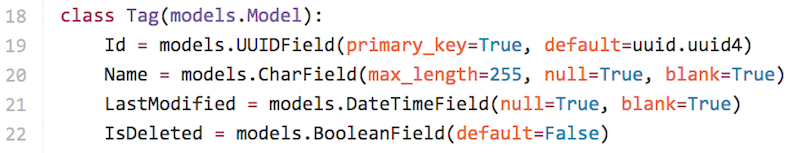
\includegraphics[scale=0.5]{pics/django_tag.png}

\vspace{0.5cm}

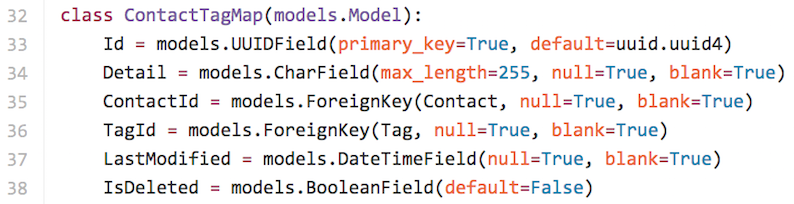
\includegraphics[scale=0.5]{pics/django_tagmap.png}

\vspace{0.5cm}

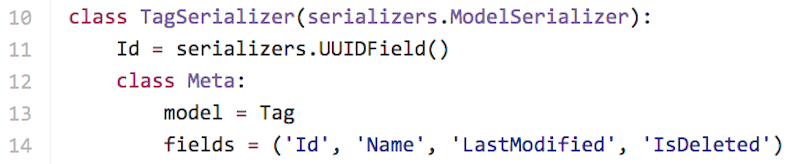
\includegraphics[scale=0.46]{pics/django_serializer.png}
%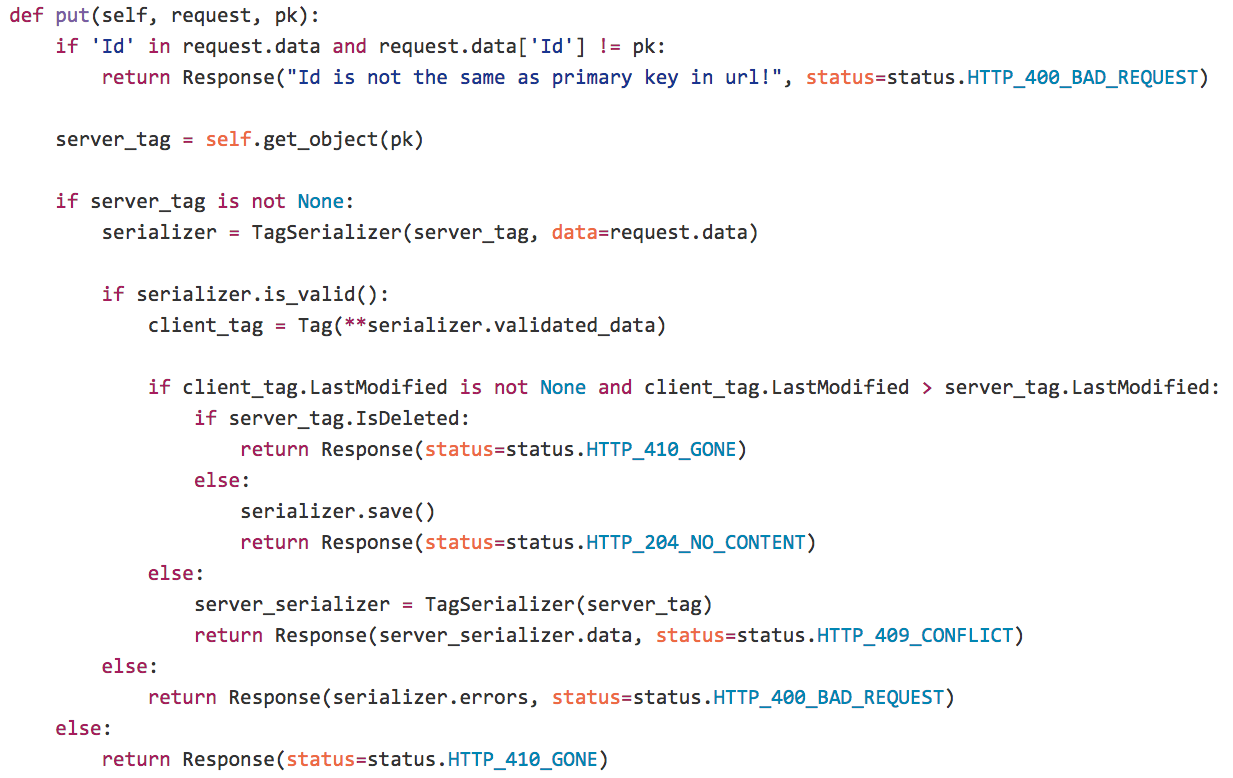
\includegraphics[scale=0.6]{pics/django_put.png}
\caption{Backend Server Implementation}\label{fg:server_implementation}
\end{centering}
\end{figure}


\subsection{Communication}
The communication between the clients and the server is achieved by using RESTful HTTP requests. The server provides an API which contains 11 endpoints, each endpoint is corresponded to a table in the database such as contacts, phone numbers, tags, relationships. An endpoint responds to the HTTP requests sent by clients differently to perform the CRUD (Create-Read-Update-Delete) operations on the database. Furthermore, to simulate the intermittent nature of the Internet, we sometimes perform an interruption to the synchronization process. Besides, while many mobile clients are being used by the users, there can be situations that some conflicts occur. Normally, the users have to manually resolve the conflicts. However, to reduce the complexity, we create a time stamp of the last modification on an entry and use it to decide which version to keep (i.e., we keep the latest version).

% To resolve the conflicts, we apply opportunistic locking to our database. The basic idea is maintaining a version for every database entry and only allowing modification if the client's entry has the same version as the server's entry, when the two entries have different versions (conflict) the user has to resolve the conflict manually
% This solution just simplifies the implementation without any significant impact on the synchronization process.

\section{Scenarios and Results}
In order to test whether our system achieves the goals, we ran it through different scenarios and evaluated the results. The default data set used in every scenario consisted of 200 contacts, each contact had 3 traditional fields: first name, phone number, and email. Additionally, there were also 100 tags attached to 100 contacts, and 100 relationships which connected 100 pairs of contacts. The details of the scenarios will be discussed in the following sections.

\subsubsection{Scenario 1: Creation}
The first scenario aimed at testing the first goal: \textit{Clients can push contact data to backend server}. Therefore, we created an initial database with the default data set in the client then started the synchronization process. This scenario tried to simulate the situation when a person uses Graphy for the first time in which he/she imports and creates a few contacts then starts the synchronization process when the Internet connection is available. Each creation or importation in Graphy is associated with a row in the database, then each row has a corresponding POST operation in the Sync Queue. It is important to note that before the first synchronization the users may also modify or delete some of their new entries. As a result, the Sync Queue may contain PUT and DELETE operations. However, in Graphy's algorithm instead of creating new PUT or DELETE operations of a new entry we inspect the actions and just modify the corresponding POST operation so there is only one POST operation for every newly created entry. Therefore, the Sync Queue for the initial database consisted of 1000 POST operations which represent all the entries in seven tables: Contacts, Phone Numbers, Emails, Tags, Contact-Tag Maps, Relationship Types, and Relationships. 

After running the scenario, our backend server had the same data as the client which was a success indicator. The results of the scenario are illustrated in \autoref{tb:ttc} and \autoref{fg:system_performance}. The results are very promising when the average time to completion of 10 tries is only 9.79 seconds. Particularly, the vast majority of the outcomes are less than 10 seconds. Furthermore, the time to completion will be significantly faster if the scenario is operated in high performance, dedicated servers. In short, the first goal of the system is achieved after examining the first scenario. The speed of the system is also acceptable because this scenario does not happen very often in real life.

\begin{table}[!ht]
\centering
\caption{Time to Completion of The Scenarios (seconds)}\label{tb:ttc}
\begin{tabular}{ | c | c | c |}
\hline
	Creation/Modification & Retrieval & Gmail Retrieval \\ \hline
	9.59 & 4.03 & 18.47 \\ \hline
	9.75 & 4.58 & 20.77 \\ \hline
	9.85 & 5.03 & 19.73 \\ \hline
	9.49 & 4.30 & 17.92 \\ \hline
	9.57 & 4.63 & 21.81 \\ \hline
	9.63 & 4.99 & 19.89 \\ \hline
	10.11 & 5.00 & 18.32 \\ \hline
	9.59 & 4.21 & 20.59 \\ \hline
	10.50 & 4.88 & 19.29 \\ \hline
	9.79 & 4.90 & 20.07 \\ \hline
        \multicolumn{3}{| l |}{\textit{Average:}} \\ \hline
        \textbf{9.79}& \textbf{4.66} & \textbf{19.69}\\ \hline
\end{tabular}
\end{table}

\subsubsection{Scenario 2: Modification}
The second scenario tried to simulate another situation in real life: a user use Graphy in the offline mode (without Internet connection). While using the application in the offline mode, the user can still perform all the actions normally. The actions are stored in the local database then synchronized with the backend server when the Internet is available. With this in mind, we made various changes to the data of the client in scenario 1 in the offline mode, then we triggered the synchronization process and waited for the data to be uploaded to the backend server. The types of changes we made included: creating new records, updating/deleting current records, and creating new tags and relationships for the existing contacts. Notably, when deleting a record, we had to delete all other related records and their operations in the Sync Queue. For example, when deleting a contact, we had to delete its phone numbers, emails, tags, relationships as well. In total, there were 90 synchronization operations needed to be transfered to the server in this scenario. We tested the scenario for 10 times and the synchronization process happened almost instantly every time (less than 1 second). Therefore, we can conclude that the modification performance is acceptable and strengthens the first goal: \textit{Clients can push contact data to backend server}.

\subsubsection{Scenario 3: Retrieval}
Nowadays, one person may own more than one device. In this scenario, we tried to simulate the case when an user starts using Graphy on another device. The new device has to connect with the server to retrieve existing data of the user to its local database. Consequently, we created an empty database in a new client then triggered the synchronization process so the new client can fetch existing data from the server. The existing data was actually the information uploaded by the first client from scenario 1 and 2. To be specific, the new client sent GET requests to all endpoints of the server's API.Each endpoint corresponded to a table in the server's database. It is important to note that we had to synchronize the table without foreign key first. For instance, the Contacts table was synchronized before the Phone Numbers table because the Phone Numbers table has a foreign key which referred to the primary key of the Contacts table. To sum up, the new client received 1000 entries from the server.

We tested the scenario 10 times and the outcomes are reported in \autoref{tb:ttc} and \autoref{fg:system_performance}. Furthermore, we ran another experiment on the Gmail Contacts service to compare its performance with our system's. The Gmail experiment was set up similarly to scenario 3. First, we created 200 contacts on Gmail then we performed the synchronization process on a new device to fetch these 200 contacts. The device we used was the Apple iPad 4 which has the Apple A6X chipset, Dual-core 1.4 GHz CPU, and 1 GB of RAM. The device operated on a Wifi network which has about 6 Mbps download speed and 1 Mbps upload speed. The Gmail experiment's results are also included in \autoref{tb:ttc} and \autoref{fg:system_performance}. From the table, we can see that the average retrieval time of Graphy is 4.66 while the retrieval time of Gmail is substantially higher at 19.69. The reason for Gmail being slower is it operated on the actual Internet connection instead of on a LAN environment like Graphy. However, as we have discussed previously, our system's hardware is far weaker than Gmail's servers. To conclude, we cannot determine that our system runs faster or slower than Gmail but we can say that it runs at an acceptable speed. Moreover, this scenario does not happen frequently, it only occurs when the user adds a new device or refresh his/her old ones. In summary, the results of this scenario has confirmed the second goal: \textit{Clients can pull contact data from backend server}.

\begin{figure}[!h]
\begin{centering}
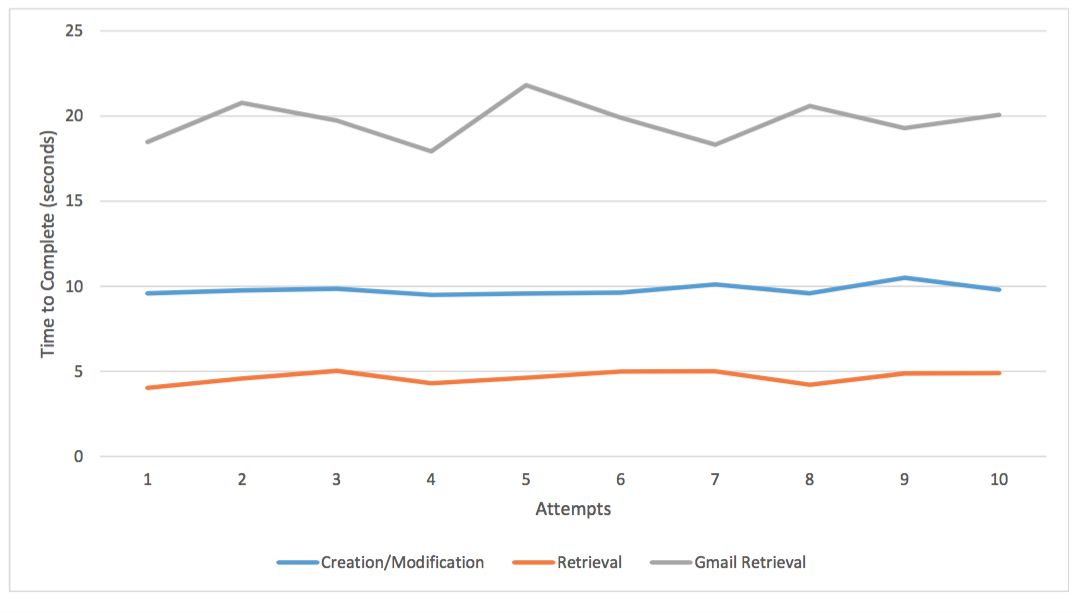
\includegraphics[scale=0.45]{pics/system_performance.png}
\caption{Time to Completion of The Scenarios}\label{fg:system_performance}
\end{centering}
\end{figure}

\subsubsection{Scenario 4: Synchronization}
This scenario addressed the third goal \textit{Clients can synchronize their contact data with each others} and the real life scenario when a person uses more than one device simultaneously. While using multiple devices at the same time, changes on one device must be propagated smoothly to other devices. In order to simulate this scenario, we used the new client in scenario 3 (i.e. client 2) and made changes to its local database. The changes were similar to the ones in scenario 2 which resulted in 90 operations in the Sync Queue. After making changes, we triggered the synchronization process on this client so the data was uploaded to the backend server. Eventually, we took the first client in scenario 2 (i.e. client 1) and started the synchronization process. We tested the scenario 10 times and the results were very positive. The database on client 1 became identical with the database on client 2, which means the synchronization algorithm worked successfully. Moreover, the process happened almost instantly (less than 1 second) in all the tests.

\subsubsection{Scenario 5: Conflicts Resolution}
In this last scenario, we wanted to tackle the final goal: \textit{Clients can resolve contact data conflicts between each others}. When a user uses many devices one at a time, it is possible that they mistakenly make different changes on the same entry multiple times on different devices. When this happens, we have a conflict to resolve. To simulate this situation, we made changes on a set of 20 entries in the database of client 1. At the same time, on client 2 we independently modified the same set of entries with different contents. After that, we triggered the synchronization function on client 1. While client 1 was synchronizing, we created an interruption so client 1 only synchronized half of its operations to the backend server. At that moment, we triggered client 2's synchronization process and let it finish completely. Therefore, at that point the server had received half of the changes from client 1 and all the changes from client 2. Eventually, we continued the synchronization process on client 1 and let it deal with the conflicts caused by client 2. The result was: client 1 resolved the conflicts and its database became identical with client 2 (client 2 made the changes at a later time compared with client 1 so its modifications took over client 1's modifications). We carried out the experiment 10 times and the resolution process always happened immediately. Therefore, we conclude that our system has achieved its final goal of being able to resolve data conflicts between devices.

%\begin{table}[!ht]
%\centering
%\caption{abc}\label{tb:abcd}
%\begin{tabular}{ | c | c | }
%\hline
%	Creation/Modification & Retrieval & Gmail Retrieval \\ \hline
%	9.5877 & 4.0301 & 18.47 \\ \hline
%	9.7471 & 4.5846 & 20.77 \\ \hline
%	9.8455 & 5.0286 & 19.73 \\ \hline
%	9.4878 & 4.2998 & 17.92 \\ \hline
%	9.5682 & 4.6329 & 21.81 \\ \hline
%	9.6295& 4.9852 & 19.89 \\ \hline
%	10.1144 & 5.0014 & 18.32 \\ \hline
%	9.5907 & 4.2031 & 20.59 \\ \hline
%	10.4971 & 4.8837 & 19.29 \\ \hline
%	9.7939& 4.9016 & 20.07 \\ \hline
%        \multicolumn{2}{| l |}{\textit{Average:}} \\ \hline
%        \textbf{9.7861}& \textbf{4.6551} & \textbf{19.686}\\ \hline
%\end{tabular}
%\end{table}

\section{Conclusion}
To sum up, according to the results of the experiment we can say that our system has achieved its goals. The data models for tags and relationships can be synchronized successfully using our algorithm. Moreover, in spite of running on a mock system with very limited computing power, the synchronization process managed to complete all the scenarios in a surprisingly short time. However, we emphasize again that our work does not focus on building the best system or creating the fastest synchronization algorithm. Therefore, the system can be optimized further when we want to deploy it to a larger environment in the future. For example, we can implement opportunistic locking strictly on the server's database to make sure the select and update functions happen in one transaction.
